Chương này trình bày những nội dung như sau:
\begin{itemize}
	\item Dữ liệu sử dụng thực nghiệm
	\item Những công cụ sử dụng trong thực nghiệm
	\item Đánh giá kết quả thực nghiệm
	\item Khả năng ứng dụng và hướng phát triển của đề tài
	\item Kết luận
\end{itemize}

\section{Dữ liệu thực nghiệm}
\label{sec:data}
\begin{center}
	\begin{figure}[htp]
		\begin{center}
			
\includegraphics[scale=.4]{codehunt1.png}
		\end{center}
		\caption{Giao diện viết chương trình}
		\label{refhinh1}
	\end{figure}
\end{center}

Code Hunt \cite{CodeHunt} là một nền tảng chơi game, được sử dụng cho các cuộc thi viết mã và thực hành các kỹ năng lập trình. Code Hunt dựa trên công cụ thực thi biểu tượng Pex. Mã Hunt là một nền tảng mã hóa trực tuyến, trong đó mỗi câu đố được trình bày với các trường hợp kiểm tra, không có đặc điểm kỹ thuật. Đầu tiên người chơi phải chọn câu hỏi và trả lời mã câu hỏi bằng cách viết một đoạn mã sao cho kết quả trùng với kết quả cử câu hỏi. Code Hunt đã được hơn 350.000 người chơi sử dụng tính đến tháng 8 năm 2016. Dữ liệu từ các cuộc thi gần đây đã được công khai và cho phép tải về tập dữ liệu này để phân tích và nghiên cứu trong cộng đồng giáo dục.


Tập dữ liệu Code Hunt chứa các chương trình do sinh viên trên toàn thế giới viết, với 250 người sử dụng, 24 câu hỏi và khoảng 13.000 chương trình được sinh viên thực hiện trên 2 ngôn ngữ là Java và C Scharp. Để có thể sử dụng tập dữ liệu Code Hunt cho đề tài của tôi, tôi đã thực hiện chuyển đổi những chương trình bằng ngôn ngữ Java thành ngôn ngữ C\#  bằng công cụ chuyển đổi của hãng Tangible Software Solutions và loại bỏ một số chương trình lỗi và không phù hợp.


\begin{center}
	\begin{figure}[htp]
		\begin{center}
			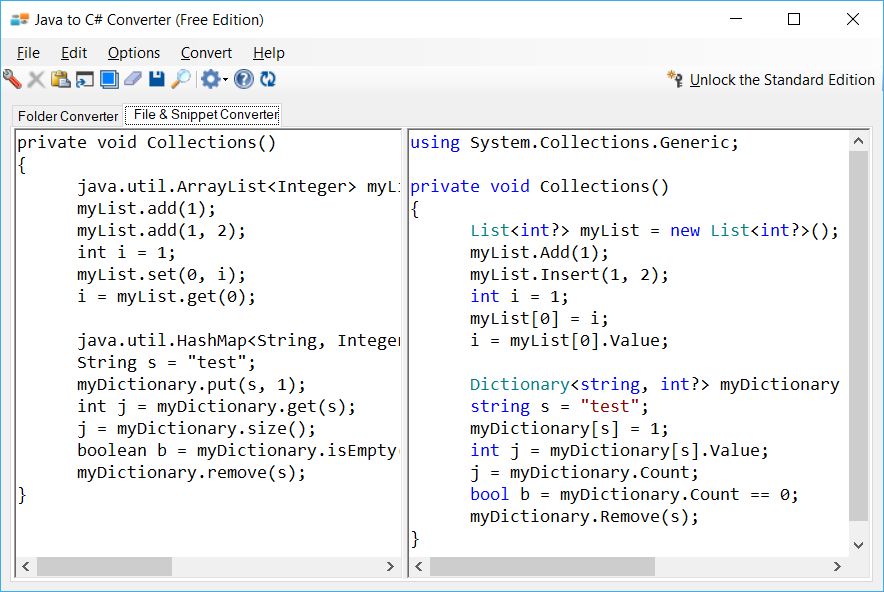
\includegraphics[scale=.4]{java-to-csharp-collections.png}
		\end{center}
		\caption{Chuyển đổi code Java sang C Scharp}
		\label{refhinh1}
	\end{figure}
\end{center}

\section{Công cụ dùng trong thực nghiệm}
%Phần này trình bày những công cụ được sử dụng để triển khai thực nghiệm như: công cụ sinh dữ liệu kiểm thử, môi trường lập trình, \dots
\subsection*{Microsoft Visual studio}
Microsoft Visual Studio là một môi trường phát triển tích hợp từ Microsoft. Nó được sử dụng để phát triển chương trình máy tính cho Microsoft Windows, cũng như các trang web, các ứng dụng web và các dịch vụ web. Visual Studio sử dụng nền tảng phát triển phần mềm của Microsoft như Windows API, Windows Forms, Windows Presentation Foundation, Windows Store và Microsoft Silverlight. Nó có thể sản xuất cả hai ngôn ngữ máy và mã số quản lý.

Visual Studio bao gồm một trình soạn thảo mã hỗ trợ IntelliSense cũng như cải tiến mã nguồn. Trình gỡ lỗi tích hợp hoạt động cả về trình gỡ lỗi mức độ mã nguồn và gỡ lỗi mức độ máy. Công cụ tích hợp khác bao gồm một mẫu thiết kế các hình thức xây dựng giao diện ứng dụng, thiết kế web, thiết kế lớp và thiết kế giản đồ cơ sở dữ liệu. Nó chấp nhận các plug-in nâng cao các chức năng ở hầu hết các cấp bao gồm thêm hỗ trợ cho các hệ thống quản lý phiên bản (như Subversion) và bổ sung thêm bộ công cụ mới như biên tập và thiết kế trực quan cho các miền ngôn ngữ cụ thể hoặc bộ công cụ dành cho các khía cạnh khác trong quy trình phát triển phần mềm.

\begin{center}
	\begin{figure}[htp]
		\begin{center}
			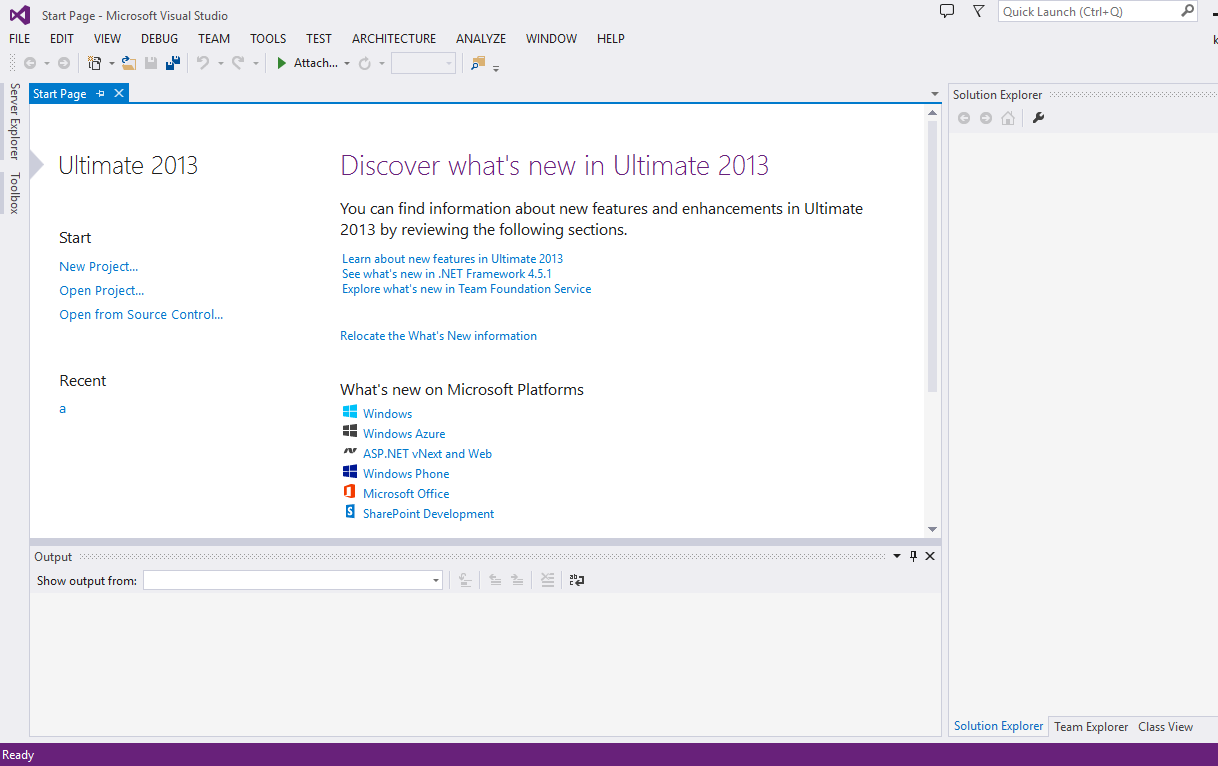
\includegraphics[scale=.4]{visualstudio.png}
		\end{center}
		\caption{Giao diện phần mềm Visual studio 2013}
		\label{refhinh1}
	\end{figure}
\end{center}

Visual Studio hỗ trợ nhiều ngôn ngữ lập trình khác nhau và cho phép trình biên tập mã và gỡ lỗi để hỗ trợ (mức độ khác nhau) hầu như mọi ngôn ngữ lập trình. Các ngôn ngữ tích hợp gồm có C,[1] C++ và C++/CLI (thông qua Visual C++), VB.NET (thông qua Visual Basic.NET), C thăng (thông qua Visual C thăng) và F thăng (như của Visual Studio 2010). Hỗ trợ cho các ngôn ngữ khác như J++/J thăng, Python và Ruby thông qua dịch vụ cài đặt riêng rẽ. Nó cũng hỗ trợ XML/XSLT, HTML/XHTML, JavaScript và CSS.

\subsection*{Ngôn ngữ lập trình C\# }
\subsubsection*{Tổng quan Ngôn ngữ C\# }
Quá trình dịch chương trình trong C\# là một ngôn ngữ lập trình hiện đại, được phát triển bởi Anders Hejlsberg cùng nhóm phát triển .Net Framework của Microsoft và được phê duyệt bởi European Computer Manufacturers Association (ECMA) và International Standards Organization (ISO).

Quá trình dịch chương trình trong C\#  được thiết kế cho các ngôn ngữ chung cơ sở hạ tầng (Common Language Infrastructure – CLI), trong đó bao gồm các mã (Executable Code) và môi trường thực thi (Runtime Environment) cho phép sử dụng các ngôn ngữ cấp cao khác nhau trên đa nền tảng máy tính và kiến trúc khác nhau.

\subsubsection*{Ngôn ngữ ra đời cùng với .NET}
\begin{itemize}
	\item Kết hợp C++ và Java.
	\item Hướng đối tượng.
	\item Hướng thành phần.
	\item Mạnh mẽ (robust) và bền vững (durable).
	\item Mọi thứ trong Quá trình dịch chương trình trong C\#  đều Object oriented.
	\item Chỉ cho phép đơn kế thừa.
	\item Lớp Object là cha của tất cả các lớp.
	\item Cho phép chia chương trình thành các thành phần nhỏ độc lập nhau.
	\item Mỗi lớp gói gọn trong một file, không cần file header như C/C++.
	\item Bổ sung khái niệm namespace để gom nhóm các lớp.
	\item Bổ sung khái niệm “property” cho các lớp.
	\item Khái niệm delegate và event.
\end{itemize}

\subsubsection*{Vai trò C\#  trong .NET Framework}
\begin{itemize}
	\item .NET runtime sẽ phổ biến và được cài trong máy client.
	\begin{enumerate}
		\item Việc cài đặt App C\#  như là tái phân phối các thành phần .NET
		\item Nhiều App thương mại sẽ được cài đặt bằng Quá trình dịch chương trình trong C\# .
	\end{enumerate}
	\item C\# tạo cơ hội cho tổ chức xây dựng các App Client/Server n-tier.
	\item Kết nối ADO.NET cho phép truy cập nhanh chóng và dễ dàng với SQL Server, Oracle…
	\item Cách tổ chức .NET cho phép hạn chế những vấn đề phiên bản.
	\item ASP.NET viết bằng Quá trình dịch chương trình trong C\#.
	\begin{enumerate}
		\item GUI thông minh.
		\item Chạy nhanh hơn (đặc tính của .NET)
		\item Mã ASP.NET không còn hỗn độn.
		\item Khả năng bẫy lỗi tốt, hỗ trợ mạnh trong quá trình xây dựng App Web.
	\end{enumerate}
\end{itemize}

\subsubsection*{Quá trình dịch chương trình trong C\# }
Mã nguồn C\# là các tập tin *.cs được trình biên dịch Compiler biên dịch thành các file *.dll hoặc *.exe, sau đó các file này được các hệ thống thông dịch CLR trên điều hành thông dịch qua mã máy và dùng kỹ thuật JIT (just-in-time) để tăng tốc độ.

\begin{center}
	\begin{figure}[htp]
		\begin{center}
			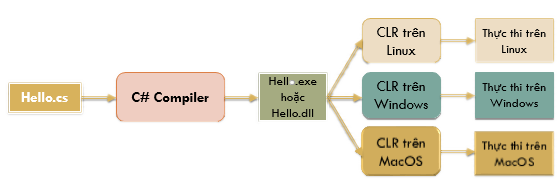
\includegraphics[scale=.4]{quatrinhthongdich.png}
		\end{center}
		\caption{Quá trình dịch chương trình trong C\#}
		
	\end{figure}
\end{center}

\subsubsection*{Các loại ứng dụng của C\#}
C\# có thể tạo ra được nhiều loại ứng dụng, trong đó có 3 kiểu phổ biến được nhiều nhà lập trình viên sử dụng nhất đó là: Console, Window và ứng dụng Web.
\begin{itemize}
	\item Ứng dụng Console là ứng dụng có giao diện text, chỉ xử lý nhập xuất trên màn hình Console, tương tự với các ứng dụng DOS trước đây. Loại ứng dụng Console thường đơn giản, ta có thể nhanh chóng tạo chương trình hiển thị kết xuất trên màn hình. Do đó, các minh hoạ, ví dụ ngắn gọn ta thường sử dụng dạng chương trình Console để thể hiện.
	\item Ứng dụng Windows Form là ứng dụng được hiển thị với giao diện cửa sổ đồ họa. Chúng ta chỉ cần kéo và thả các điều khiển (control) lên cửa sổ Form. Visual Studio sẽ sinh mã trong chương trình để tạo ra, hiển thị các thành phần trên cửa sổ.
	\item Ứng dụng Web, trên môi trường .NET cung cấp công nghệ ASP.NET, MVC giúp xây dựng những trang Web động. Để tạo ra một trang Web, người lập trình sử dụng ngôn ngữ biên dịch như C\# hoặc C\# để viết mã. Để đơn giản hóa quá trình xây dựng giao diện người dùng cho trang Web, .NET giới thiệu công nghệ Webform. Cách thức tạo ra các Web control tương tự như khi ta xây dựng ứng dụng trên Window Form.
\end{itemize}

\subsection{Công cụ sinh dữ liệu thử Pex}
\subsubsection*{Giới thiệu}
Khái niệm về DSE và các ứng dụng sử dụng kỹ thuật DSE đã có từ lâu, nhưng Pex là một ứng dụng mỡ rộng hơn so với các phiên bản DSE trước. Trong Visual Stuio, Pex đã được tích hợp như một Add-in, và có thể tạo ra các test case kết hợp với các bộ kiểm thử khác nhau như NUnit và MSTest. 

Cũng như với Unit Test, ta có thể viết các lớp kiểm thử chứa các ca kiểm thử tham số hóa. Với sự hỗ trợ của Pex ta có thể thực thi các ca kiểm thử tham số hóa đó. Tuy nhiên không giống việc thực thi các lớp kiểm thử chứa các Unit Test, Pex chỉ thực thi được một ca kiểm thử tham số hóa trong mỗi lần chạy.

\begin{lstlisting}[language={[Sharp]C}, caption={Ca kiểm thử tham số sử dụng Pex}, label={Script}]
[PexMethod]
public void AddSpec(ArrayList list, object element) {
// assumptions
PexAssume.IsTrue(list != null);
// method sequence
int len = list.Count; 
list.Add(element);
// assertions
Assert.IsTrue(list[len] == element);
}
\end{lstlisting}


\subsubsection*{Các mẫu kiểm thử tham số hóa}
Viết các ca kiểm thử các tham số là một công việc tốn nhiều công sức. Để viết các ca kiểm thử các tham số hiệu quả, ta cần thực sự hiểu về mã cài đặt của chương trình mà ta muốn kiểm thử. Pex hỗ trợ cho chúng ta nhiều mẫu kiểm thử tham số khác nhau \cite{de2008parameterized}. Các mẫu được sử dụng nhiều nhất đó là mẫu AAA (Triple-A) và AAAA:
\begin{itemize}
	\item Với mẫu AAA (Arrange, Act, Assert) PUT được tổ chức thành 3 phần:
	\begin{itemize}
		\item Arrange: khởi tạo giá trị các biến sẽ sử dụng
		\item Act: dãy các lời gọi phương thức
		\item Assert: sự xác nhận
	\end{itemize}
	\item Với mẫu AAAA, một giả thuyết (Assume) được thêm vào để giới hạn miền giá trị của các tham số đầu vào.
\end{itemize}

\begin{lstlisting}[language={[Sharp]C}, caption={Mầu kiềm thử tham số hóa AAAA}, label={Script}]
[PexMethod]
void AssumeActAssert(ArrayList list, object item) { 
// assume
PexAssume.IsNotNull(list);
// arrange
var count = list.Count;
// act
list.Add(item);
// assert
Assert.IsTrue(list.Count == count + 1);
}
\end{lstlisting}

\subsubsection*{Lọn chọn đầu vào kiểm thử với Pex}
Đổ có thể sinh các đầu vào cụ thể cho các tham số Unit test, Pex cần phải phân tích chương trình với các tham số kiểm thử này. Có 2 kỹ thuật phân tích chương trình đó là:

\begin{itemize}
	\item Phân tích tĩnh (static analysis): Kiểm chứng một tính chất nào đó của chương trình bằng việc phân tích tất cả các đường đi thực thi. Kỹ thuật này coi các cảnh bảo (violations) là các lỗi (error).
	\item Phân tích động (dynamic analysis): Kiểm chứng một tính chất bằng việc phân tích một số đường đi thực thi. Đây là một kỹ thuật phân tích động hỗ trợ việc phát hiện ra các lỗi (bugs) nhưng không khẳng định được rằng có còn những lỗi khác hay không. Các kỹ thuật này thường không tìm ra được tất cả các lỗi.
\end{itemize}

Pex cài đặt một kỹ thuật phân tích chương trình bằng cách kết họp cả hai kỹ thuật phân tích chương trình ở trên gọi là thực thi tượng trưng động \cite{xie2009fitness}, \cite{godefroid2005dart}. Về bản chất Pex là một công cụ hỗ trợ kỹ thuật kiểm thử hộp hắng (white-box testing). Tương tự như kỹ thuật phân tích chương trình tĩnh, Pex chứng minh được rằng một tính chất được kiểm chứng trong tất cả các đường đi khả thi. Pex chỉ báo cáo (reporting) về các lỗi thực sự như với kỹ thuật phân tích chương trình động.

Pex sử dụng bộ xử lý ràng buộc Z3 \cite{de2008z3} kết họp với các lý thuyết toán học khác như hàm chưa định nghĩa, lý thuyết mảng, bit-vetor \cite{kroening2016decision} để giải quyết ràng buộc sinh ra trong quá trình thực thi tượng trưng động và sinh ra các đầu vào kiểm thử cụ thể cho tham số kiểm thử.

\subsubsection*{Mô hình ứng dụng Pex}

\begin{center}
	\begin{figure}[htp]
		\begin{center}
			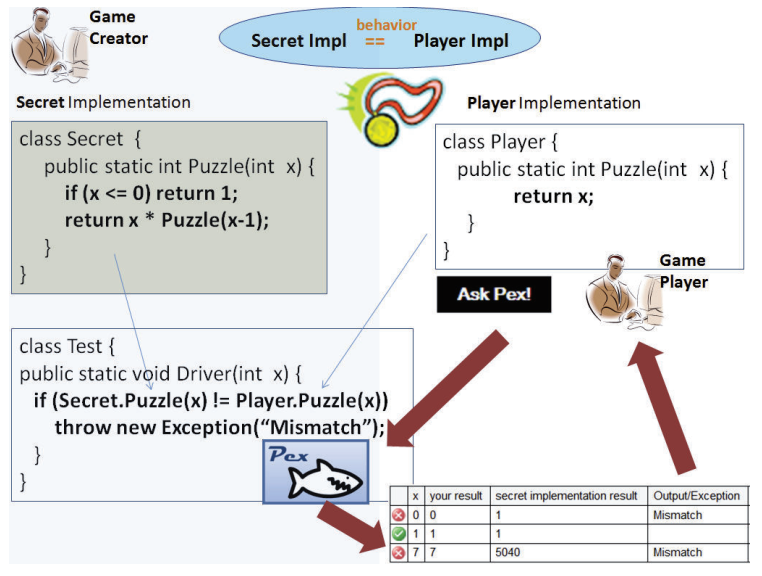
\includegraphics[scale=.4]{pex.png}
		\end{center}
		\caption{Mô hình ứng dụng Pex}
		
	\end{figure}
\end{center}

\section{Đánh giá kết quả thực nghiệm}
Phần này trình bày những kết quả đo được trên bộ dữ liệu thực nghiệm đã nêu trong Phần~\ref{sec:data}.

\section{Khả năng ứng dụng}
Phần này trình bày một số ứng dụng có thể của việc đo độ tương tự về hành vi của chương trình cùng hướng phát triển trong tương lai.

\subsection{Đánh giá tiến bộ trong lập trình}
Theo dõi sự tiến bộ trong học tập là một việc quan trọng, mà ngay cả với giảng viên và sinh viên công việc này là cả một quá trình. Có nhiều tiêu chí đánh giá sự tiến bộ trong học tập của sinh viên, trong đó tiêu chí về điểm số là một trong những tiêu chí cơ bản nhất. Một bảng thống kê điểm số, thành tích học tập của sinh viên sẽ thể hiện được sự tiến bộ của sinh viên trong học tập. Nhưng công việc chấm bài, tổng hợp, thống kê kết quả học tập của sinh viên mất rất nhiều thời gian của giảng viên. Một ứng dụng hỗ trợ chấm điểm, lưu trữ, thống kê và đánh giá điểm số của sinh viên là sẽ là một công cụ hỗ trợ đắc lực cho giảng viên trong công tác quản lý của mình. Nếu số liệu thống kê đánh giá kết quả các bài kiểm tra của sinh viên ngày càng cao, chứng tỏ sinh viên nắm được nội dung và kiến thức của chương trình đào tạo, và kết quả tốt sẽ là một động lực giúp cho sinh viên thêm tự tin, đam mê công việc học tập của mình. Ngược lại, nếu một sinh viên có điểm số ngày càng thấp chứng tỏ sinh viên đang có vấn đề trong kiến thức của của mình, lúc này tốt nhất sinh viên nên dừng lại không tiếp tục code và kiểm tra xem vấn đề mình đang gặp phải. 

\subsection{Xếp hạng tự động}
Công việc chấm điểm, phân loại và xếp hạng các bài kiểm tra của sinh viên cũng là một công việc tốn không ít công sức của giảng viên. Để giảm bớt gánh nặng cho giảng viên, chúng ta có thể sử dụng kết quả các độ đo trên từng bài tập của sinh viên như một phương pháp hỗ trợ công việc chấm điểm của từng sinh viên. Sự giống nhau về hành vi giữa chương trình của sinh viên và chương trình tham chiếu có thể là một yếu tố để phân loại sinh viên. Độ tương tự càng cao thì điểm số càng cao, các chỉ số này dựa hoàn toàn trên ngữ nghĩa của chương trình. Cách tiếp cận này giải quyết được các giới hạn trong trường hợp chương trình của sinh viên giống với chương trình tham chiếu, nhưng khác nhau về ngữ nghĩa. Các kết quả trong việc xếp hạng tự động sẽ giúp tiết kiệm được thời gian và giảng viên có thể đưa ra giải pháp giúp những sinh viên có điểm số thấp khắc phục được hạn chế đang gặp phải.

\subsection{Gợi ý giải pháp lập trình}
Thông thường, sinh viên thường viết code mới thực hiện chạy chương trình, lúc này sinh viên mới biết được kết quả đoạn code vừa thực hiện. Để hỗ trợ sinh viên viết code được tốt hơn, nếu như có một công cụ hỗ trợ kiểm tra theo thời gian thực và gửi thông báo lỗi nếu sinh viên viết code sai cú pháp hoặc chương trình bị lỗi không thể thực thi được. Ngoài ra, công cụ sẽ gợi ý giải pháp lập trình cho sinh viên bằng hình thức tự động tính toán thông báo kết quả các tham số đầu vào và đầu ra của chương trình so với chương trình được tham chiếu, đưa ra các số liệu về độ tương tự hành vi của chương trình.	

\subsection{Hướng phát triển}
Qua quá trình nghiên cứu và triển khai thực nghiệm, trong tương lai đề tài hướng tới phát triển thành một một ứng dụng hoàn chỉnh với việc bổ sung và hoàn thiện một số chức năng như sau:
\begin{itemize}
	\item Phát triển ứng dụng có thể chạy trên Web
	\item Chức năng quản lý sinh viên
	\item Quản lý kết quả học tập sinh viên
	\item Thêm chức năng đánh giá, xếp hạng tự động
	\item Thêm chức năng gợi ý giải pháp lập trình
	\item Cải tiến các độ đo để cho kết quả tốt hơn và nhanh hơn
	\item Phát triển thêm các nền tảng lập trình khác như java, c++..		
\end{itemize}

\section{Kết luận}
Qua quá trình nghiên cứu đề tài, có thể thấy rằng việc phát triển và ứng dụng các kỹ thuật đo đang dần trở nên phổ biến trong các chương trình giáo dục và đào tạo lập trình viên online. Những lợi ích, hiểu quả của việc đánh giá độ tương tự hành vi mang lại là rất thiết thực. Các kỹ thuật này không chỉ giúp quá trình giảng dạy của giảng viên được thuận lợi hơn, tiết kiệm được thời gian cũng như công sức trong công tác quản lý. Ngoài ra, sinh viên có được một môi trường tốt để tự rèn luyện, nâng cao các kỹ năng lập trình của bản thân. Việc tạo động lực giúp sinh viên có sự hứng thú và đam mê lập trình là rất cần thiết. Một khi sinh viên có tư duy và kỹ năng lập trình tốt, sinh viên sẽ tự tin vào năng lực của bản thân để tiếp tục phát phát triển sự nghiệp sau khi ra trường.

Đề tài đã thực hiện nghiên cứu rất nhiều vấn đề, nhưng trọng tâm đó là nghiên cứu sơ lượt về công cụ PEX của Microsoft, một công cụ sử dụng bộ xử lý ràng buộc Z3 \cite{de2008z3} kết họp với các lý thuyết toán học khác như hàm chưa định nghĩa, lý thuyết mảng, bit-vetor \cite{kroening2016decision} để giải quyết các ràng buộc sinh ra trong quá trình thực thi tượng trưng động, và sinh ra các đầu vào kiểm thử có độ phủ cao cho tham số kiểm thử của chương trình. Ứng dụng công cụ PEX nghiên cứu các kỹ thuật đo độ tương tự hành vi của chương trình, sao cho kết quả các độ đo được chính xác hơn. Từ khả năng xử lý của các độ đo, xây dựng một công cụ để minh họa cho các kỹ thuật đo.

Những nội dung trình bày trong luận văn này không tránh khỏi còn nhiều thiếu xót vì lý do nhiều lý do khách quan khác nhau như: Thời gian thực hiện đề tài hạn hẹp; lượng kiến thức cơ sở để triển khai thực hiện rất lớn; cùng với đó là kinh nghiệm của bản thân trong việc thực hiện các đề tài chưa có. Tuy nhiên, với sự hướng dẫn tận tình của giáo viên hướng dẫn, đề tài đã đạt được nhiều nội dung quan trọng, và có thể mở ra nhiều hướng nghiên cứu và phát triển khác của đề tài. Như việc mở rộng DSE để hỗ trợ việc thực thi tượng trưng các chương trình có dữ liệu phức tạp, hay có số vòng lặp lớn. Cải tiến kỹ thuật đo, kết hợp với kỹ thuật DSE để có kết quả độ đo được chính xác hơn, nhạy hơn. Tiếp tục nghiên cứu, phát triển để thực các kỹ thuật đo trên các ngôn ngữ khác như Java, C++ và chạy được trên nền tảng PC, Web. 

